\documentclass[a4paper]{article}
\usepackage[utf8x]{inputenc}
\usepackage[T1]{fontenc}
\usepackage[MeX]{polski}
\usepackage{amssymb}
\usepackage{graphicx}
\usepackage{fancyhdr}
\usepackage{lastpage}
\usepackage{xcolor}
\usepackage{color, colortbl}
\usepackage{hyperref}
\definecolor{tableofcontents}{RGB}{0, 0, 0}
\hypersetup{
    colorlinks=true,
    urlcolor=blue,
    linkcolor=tableofcontents,
}


\pagestyle{fancy}
\fancyhf{}
\cfoot{ \thepage \hspace{1pt} / \pageref{LastPage}}
\lhead{Specyfikacja funkcjonalna}
\rhead{\texttt{War Of Tanks}}


\begin{document}

\begin{titlepage}
	\begin{center}
		\vspace*{5cm}

	        \Huge
        	\textbf{Specyfikacja funkcjonalna}

        	\vspace{1cm}
	        \Huge
        	\texttt{War Of Tanks}

    		\vspace{1.5cm}

	        \large
		    Aleksandra Michalska, Natalia Olszewska

        	\vfill

	        \vspace{3cm}

		\large 24.04.2021
	\end{center}
\end{titlepage}

\tableofcontents

\newpage



\section{Informacje og\'olne}

\subsection{O dokumencie}
\quad Dokument koresponduje z dokumentem \textit{"Specyfikacja Implementacyjna"}. 
Ma na celu przybli\.zenie korzystania z programu jego u\.zytkownikowi docelowemu.
\subsubsection{U\.zytkownik docelowy}
\quad Program jest powszechnie dost\k{e}pny oraz dedykowany jest dla ka\.zdego u\.zytkownika.

\subsection{Cel projektu}
\quad Celem projektu jest napisanie gry na jedno urz\k{a}dzenie dla dw\'och u\.zytkownik\'ow. 










\section{Informacje o programie}

\subsection{Nazwa programu}
\quad Nazwa programu to \texttt{\textit{"War Of Tanks"}}. 

\subsection{Dost\k{e}pno\'s\'c}
\quad Program dost\k{e}pny jest na systemy operacyjne Microsoft Windows, Linux (dystrybuje Ubuntu oraz Mint) oraz Mac OS.

\subsection{Opis programu}
\quad Program jest przeznaczony dla dw\'och graczy korzystaj\k{a}cych z jednego urz\k{a}dzenia. 
W grze \texttt{\textit{"War Of Tanks"}} u\.zytkownicy poruszaj\k{a} si\k{e} czo\l{}gami z ruchomymi lufami u\.zywaj\k{a}c klawiatury (patrz sekcja \textit{"Ruch czo\l{}gu"}).
Ich zadaniem jest strzelanie do spadaj\k{a}cych kom\'orek, ich kolonii oraz nieruchomej kom\'orki-bomby.
Rozgrywka ko\'nczy si\k{e} w momencie zestrzelenia kom\'orki-bomby lub w przypadku up\l{}yni\k{e}cia ustalonej ilo\'sci czasu.
Gr\k{e} wygrywa osoba, kt\'ora w momencie jej zako\'nczenia posiada wi\k{e}ksz\k{a} ilo\'s\'c punkt\'ow.

\subsubsection{U\.zytkownik docelowy}
\quad Program jest powszechnie dost\k{e}pny oraz dedykowany dla ka\.zdego u\.zytkownika.








\section{Opis funkcjonalno\'sci}


\subsection{Uruchomienie programu}
\quad Uruchomienie programu odbywa si\k{e} przy u\.zyciu konsoli systemowej lub odpowiednich program\'ow (np. IntelliJ, NetBeans).

\subsection{Parametry programu}
\begin{itemize}
    \item \texttt{\textbf{v1}} - pocz\k{a}tkowa pr\k{e}dko\'s\'c pocisk\'ow wystrzeliwanych przez czo\l{}gi (w pikselach na sekund\k{e})
    \item \texttt{\textbf{x1}} - maksymalna ilość pocisk\'ow jednego gracza, jaka mo\.ze istnie\'c jednocze\'snie (tak długo jak pocisk nie dotrze do celu lub nie wyjdzie poza planszę, uznaje się, że pocisk istnieje)
    \item \texttt{\textbf{r1}} - pocz\k{a}tkowy promie\'n pocisku (w pikselach)
    \item \texttt{\textbf{v2}} - pocz\k{a}tkowa prędko\'s\'c spadania kom\'orek (w pikselach na sekund\k{e})
    \item \texttt{\textbf{h1}} - pocz\k{a}tkowa długo\'s\'c boku kwadratu kom\'orki (w pikselach)
    \item \texttt{\textbf{p1}} - pocz\k{a}tkowa warto\'s\'c kom\'orki (w ilo\'sci pocisk\'ow potrzebnych do zabicia kom\'orki)
    \item \texttt{\textbf{t1}} - czas (w sekundach), po kt\'orym zmienia\'c si\k{e} b\k{e}d\k{a} nast\k{e}puj\k{a}ce parametry:
    \begin{itemize}
        \item[$\diamond$] \texttt{\textbf{dv1}} - zwi\k{e}kszenie pr\k{e}dko\'sci poruszania si\k{e} pocisk\'ow (w pikselach na sekund\k{e})
        \item[$\diamond$] \texttt{\textbf{dv2}} - zwi\k{e}kszenie pr\k{e}dko\'sci poruszania si\k{e} kom\'orek (w pikselach na sekund\k{e}) 
        \item[$\diamond$] \texttt{\textbf{dr1}} - zmniejszenie promienia kuli o podan\k{a} warto\'s\'c (w pikselach)
        \item[$\diamond$] \texttt{\textbf{dh1}} - zmniejszenie rozmiaru boku kom\'orki (w pikselach)
    \end{itemize}
    \item \texttt{\textbf{t2}} - czas (w sekundach), po kt\'orym zwi\k{e}ksza\'c b\k{e}dzie si\k{e} bie\.z\k{a}ca warto\'s\'c kom\'orek o 1
    \item \texttt{\textbf{t3}} - czas trwania gry (w minutach)
\end{itemize}

\subsection{Jak korzysta\'c z programu?}

\subsubsection{Panel startowy}
\quad Po uruchomieniu programu, wy\'swietla si\k{e} panel startowy. W tym miejscu u\.zytkownik mo\.ze:
\begin{itemize}
    \item uruchomi\'c gr\k{e} za pomoc\k{a} przycisku \texttt{START},
    \item przej\'s\'c do ustawie\'n d\'zwi\k{e}ku za pomoc\k{a} przycisku \texttt{SETTINGS} (patrz sekcja \textit{"Panel ustawie\'n"}),
    \item przekaza\'c plik konfiguracyjny w menu \texttt{AddConfigurationFile} (patrz sekcje \textit{"Plik konfiguracyjny"} oraz \textit{"Dane wej\'sciowe"}),
    \item wy\'swietli\'c regu\l{}y gry z menu \texttt{HELP}.
\end{itemize}

\subsubsection{Plik konfiguracyjny}
\quad U\.zytkownik ma mo\.zliwo\'s\'c dostosowania dzia\l{}ania programu do w\l{}asnych preferencji, dzi\k{e}ki plikowi konfiguracyjnemu (u\.zycie: patrz sekcja \textit{"Dane wej\'sciowe"}).
Przekazanie pliku konfiguracyjnego do programu odbywa si\k{e} przez menu \\ \texttt{AddConfigurationFile}.

\subsubsection{Domy\'slne warto\'sci parametr\'ow programu}
\quad W przypadku nieskorzystania z pliku konfiguracyjnego, warto\'sci parametr\'ow programu (patrz sekcja \textit{"Parametry programu"}) zostają ustalone automatycznie (patrz Tabela \ref{table:ta}).
\begin{table}[ht]
\centering
    \renewcommand{\arraystretch}{1.3}
    \begin{tabular}{|c|c|}
    \rowcolor{lightgray}
        \hline
        parametr&warto\'s\'c \\
        \hline
        v1&10\\
        \hline
        dv1&3\\
        \hline
        v2&14\\
        \hline
        dv2&4\\
        \hline
        t1&60\\
        \hline
        t2&100\\
        \hline
        t3&5\\
        \hline
\end{tabular}
\quad
    \begin{tabular}{|c|c|}
    \rowcolor{lightgray}
        \hline 
        parametr&warto\'s\'c\\
        \hline
        x1&15\\ 
        \hline
        p1&3\\
        \hline
        r1&20\\
        \hline
        dr1&2\\
        \hline
        h1&50\\
        \hline
        dh1&3\\
        \hline
\end{tabular}
\color{lightgray}\caption{Domy\'slne warto\'sci parametr\'ow programu}
\label{table:ta}
\end{table}


\subsubsection{Panel ustawie\'n}
\quad W tym miejscu u\.zytkownik mo\.ze zmieni\'c poziom g\l{}o\'sno\'sci d\'zwi\k{e}ku programu.

\subsubsection{Panel gry}
\quad Panel gry wy\'swietlany jest po naci\'sni\k{e}ciu przycisku \texttt{START} w panelu startowym (patrz sekcja \textit{"Panel startowy"}). 
Szkic panelu gry:
\begin{figure}[ht]
    \centering
    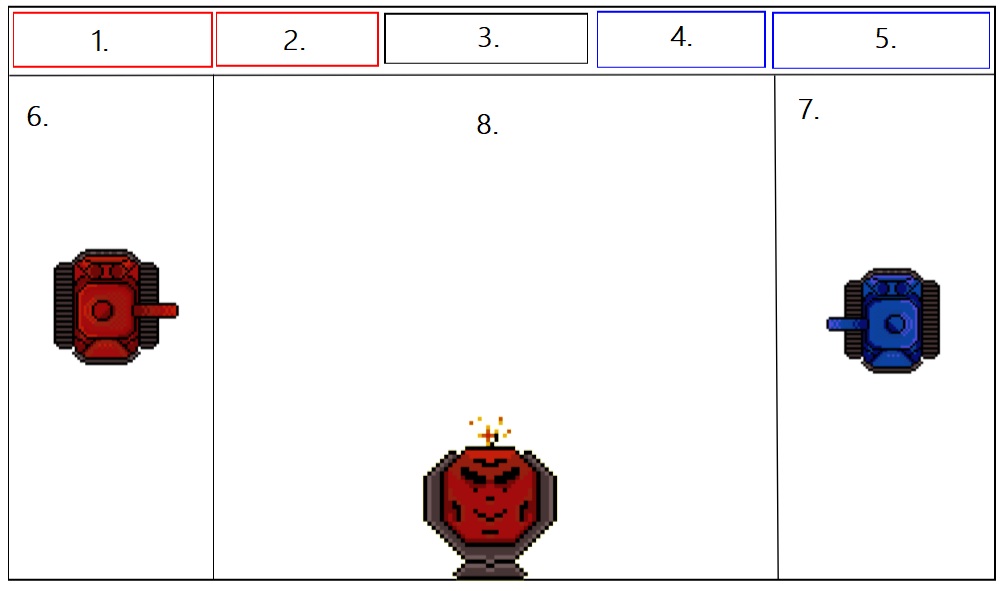
\includegraphics[scale=0.4]{exampleGamePanel.png}
    \color{lightgray}\caption{Szkic panelu gry}
    \label{fig:gamePanel}
\end{figure}


W miejscach oznaczonych cyframi znajduj\k{a} si\k{e}:
\begin{itemize}
    \item pola \textbf{1.} oraz \textbf{5.} zawieraj\k{a} ilo\'s\'c punkt\'ow odpowiednio gracza czerwonego oraz niebieskiego, 
    \item pola \textbf{2.} oraz \textbf{4.} zawieraj\k{a} ilo\'s\'c istniej\k{a}cych pocisk\'ow odpowiednio gracza czerwonego oraz niebieskiego, 
    \item pole \textbf{3.} zawiera zegar odliczaj\k{a}cy czas do zako\'nczenia rozgrywki,
    \item pola \textbf{6.} oraz \textbf{7.} wyznaczaj\k{a} obr\k{e}by, w kt\'orych mog\k{a} porusza\'c si\k{e} czo\l{}gi,
    \item pole \textbf{8.} zawiera miejsce, w kt\'orym znajduj\k{a} si\k{e} spadaj\k{a}ce kom\'orki.
\end{itemize}

\subsubsection{Ruch czo\l{}gu}
\quad Czo\l{}gi poruszaj\k{a} si\k{e} tylko po polach \textbf{6.} oraz \textbf{7.} (patrz Rysunek \ref{fig:gamePanel}).
Ruch czo\l{}gu dla gracza:
\begin{itemize}
    \item po lewej stronie (czerwony czo\l{}g):
    \begin{itemize}
        \item[$\diamond$] ruch w g\'or\k{e}: klawisz \textbf{W}
        \item[$\diamond$] ruch w d\'o\l{}: klawisz \textbf{S}
        \item[$\diamond$] obr\'ot lufy w g\'or\k{e}: klawisz \textbf{A}
        \item[$\diamond$] obr\'ot lufy w d\'o\l{}: klawisz \textbf{D}
    \end{itemize}
    \item po prawej stronie (niebieski czo\l{}g):
    \begin{itemize}
        \item[$\diamond$] ruch w g\'or\k{e}: klawisz \textbf{$\uparrow$}
        \item[$\diamond$] ruch w d\'o\l{}: klawisz \textbf{$\downarrow$}
        \item[$\diamond$] obr\'ot lufy w g\'or\k{e}: klawisz \textbf{$\leftarrow$}
        \item[$\diamond$] obr\'ot lufy w d\'o\l{}: klawisz \textbf{$\rightarrow$}
    \end{itemize}
\end{itemize}

Pr\k{e}dko\'s\'c ruchu czo\l{}gu oraz jej zmiana w trakcie gry, ustalane s\k{a} w programie (patrz sekcja \textit{"Domy\'slne warto\'sci parametr\'ow programu"}) lub przez gracza (patrz sekcja \textit{"Plik konfiguracyjny"}). 

\subsubsection{Strzelanie}
\quad Strzelanie pociskami dla gracza:
\begin{itemize}
    \item po lewej stronie (czerwony czo\l{}g): klawisz \textbf{spacja}
    \item po prawej stronie (niebieski czo\l{}g): klawisz \textbf{enter}
\end{itemize}

Maksymalna ilość pocisk\'ow jednego gracza, jaka mo\.ze istnie\'c jednocze\'snie, ustalona jest w programie (patrz sekcja \textit{"Domy\'slne warto\'sci parametr\'ow programu"}) lub przez gracza (patrz sekcja \textit{"Plik konfiguracyjny"}).

\subsubsection{Kom\'orki oraz kolonie}
\quad W polu \textbf{8.} (patrz Rysunek \ref{fig:gamePanel}) znajduj\k{a} si\k{e} spadaj\k{a}ce kom\'orki oraz ich kolonie.
Ka\.zda kolonia z\l{}o\.zona mo\.ze by\'c z 2, 3, 4 lub 5 kom\'orek. Ka\.zdej kom\'orce przypisana jest warto\'s\'c, kt\'ora odpowiada ilo\'sci pocisk\'ow potrzebnych do jej zestrzelenia.

\subsubsection{Kom\'orka-bomba}
\quad Kom\'orka-bomba jest nieruchoma i znajduje si\k{e} w dolnej cz\k{e}\'sci panelu gry. 

Do zestrzelenia kom\'orki-bomby, potrzebne jest 50 pocisk\'ow, przy czym gracz mo\.ze zadawa\'c obra\.zenia strzelaj\k{a}c wy\l{}\k{a}cznie w jej g\'orn\k{a} kraw\k{e}d\'z (pozosta\l{}e kraw\k{e}dzie s\k{a} pancerne).

Gracz, kt\'ory zada ostatnei obra\.zenie zdobywa kom\'ork\k{e}-bomb\k{e} i wygrywa gr\k{e}.

\subsubsection{Zdobywanie punkt\'ow}
\quad Gracze zdobywaj\k{a} punkty za zestrzelenie kom\'orek lub kolonii kom\'orek, przy czym:
\begin{enumerate}
    \item Za zestrzelenie kom\'orki/kolonii, punkty otrzymuje gracz, kt\'ory zada ostateczne uderzenie.
    \item Ilo\'s\'c punkt\'ow otrzymanych za zestrzelenie kom\'orki/kolonii odpowiada jej warto\'sci pocz\k{a}tkowej.
\end{enumerate}






\section{Format danych i struktura plik\'ow}

\subsection{Dane wej\'sciowe}
\quad Dane wej\'sciowe przekazywane s\k{a} w postaci pliku konfiguracyjnego (plik tekstowy o rozszerzeniu \textbf{txt}). 


W pliku konfiguracyjnym powinien znajdowa\'c si\k{e} przynajmniej jeden parametr programu (parametry programu: patrz sekcja \textit{"Parametry programu"}).  


U\.zytkownik nie ma obowi\k{a}zku przekazania do programu pliku konfiguracyjnego. W takim przypadku, warto\'sci parametr\'ow programu zostaj\k{a} ustalone jak opisano w sekcji \textit{"Domy\'slne warto\'sci parametr\'ow programu"}.

\subsubsection{Ograniczenia dla danych wej\'sciowych}
\quad Dane wej\'sciowe powinny spe\l{}nia\'c warunki przedstawione w Tabeli \ref{table:ograniczenia}.
\begin{table}[ht]
\centering
    \renewcommand{\arraystretch}{1.5}
    \begin{tabular}{|c|c|}
    \rowcolor{lightgray}
        \hline
        parametr&ograniczenie \\
        \hline
        v1& \(10 \leqslant v1 \leqslant 50\)\\
        \hline
        dv1& \(0 \leqslant dv1 \leqslant 25\)\\
        \hline
        v2& \(5 \leqslant v2 \leqslant 35\)\\
        \hline
        dv2& \(0 \leqslant dv2 \leqslant 20\)\\
        \hline
        t1& \(30 \leqslant t1 \leqslant  \frac{t3 \cdot 60}{2} \)\\
        \hline
        t2& \(30 \leqslant t2 \leqslant \frac{t3 \cdot 60}{2}\)\\
        \hline
        t3& \(3 \leqslant t3 \leqslant 15\)\\
        \hline
\end{tabular}
\quad
    \begin{tabular}{|c|c|}
    \rowcolor{lightgray}
        \hline 
        parametr&ograniczenie \\
        \hline
        x1& \(5 \leqslant x1 \leqslant 20\)\\ 
        \hline
        p1& \(1 \leqslant p1 \leqslant 9\)\\
        \hline
        r1& \(20 \leqslant r1 \leqslant 40\)\\
        \hline
        dr1& \(2 \leqslant dr1 \leqslant 10\)\\
        \hline
        h1& \(20 \leqslant h1 \leqslant 70\)\\
        \hline
        dh1& \(1 \leqslant dh1 \leqslant 10\)\\
        \hline
\end{tabular}
\color{lightgray}\caption{Domy\'slne warto\'sci parametr\'ow programu}
\label{table:ograniczenia}
\end{table}

\subsubsection{Przyk\l{}adowe dane wej\'sciowe}
Przyk\l{}adowy plik konfiguracyjny:
\begin{center}
\texttt{\textbf{-t3 8 -v1 30 -h1 60}}    
\end{center}
oznacza zmian\k{e} czasu trwania gry na \textbf{8 minut}, pr\k{e}dko\'sci pocz\k{a}tkowej pocisk\'ow na \textbf{30 pikseli} na sekund\k{e} oraz pocz\k{a}tkowej długo\'sci boku kwadratu kom\'orki na \textbf{60 pikseli}. Warto\'sci pozosta\l{}ych parametr\'ow pozostaj\k{a} niezmienione (patrz sekcja \textit{"Domy\'slne warto\'sci parametr\'ow programu"}).



\subsection{Dane wyj\'sciowe}
\quad Po zako\'nczeniu rozgrywki, zrzut ekranu okna gry zapisywany jest do pliku graficznego o rozszerzeniu \textbf{jpg}.


\section{Scenariusz dzia\l{}ania programu}

\subsection{Scenariusz og\'olny}
\quad Scenariusz og\'olny zak\l{}ada nieskorzystanie z pliku konfiguracyjnego.
\begin{enumerate}
    \item Uruchomienie
    
        U\.zytkownicy uruchamiaj\k{a} program (patrz sekcja \textit{"Uruchomienie programu"}).
    \item Pocz\k{a}tek gry
    
        U\.zytkownicy wybieraj\k{a} w panelu startowym przycisk \texttt{START}.
    \item Rozgrywka
    
        U\.zytkownicy poruszaj\k{a} si\k{e} czo\l{}gami i stzrelaj\k{a} do kom\'orek.
    \item Zako\'nczenie rozgrywki
    
        Po zako\'nczeniu czasu lub zestrzeleniu kom\'orki-bomby, rozgrywk\k{e} wygrywa u\.zytkownik z wi\k{e}ksz\k{a} ilo\'sci\k{a} punkt\'ow.
\end{enumerate}

\subsection{Scenariusz szczeg\'o\l{}owy}
\quad Scenariusz szczeg\'o\l{}owy zak\l{}ada skorzystanie z poprawnie utworzonego pliku konfiguracyjnego.
\begin{enumerate}
    \item Utworzenie i przekazanie pliku konfiguracyjengo
    
        U\.zytkownicy tworz\k{a} poprawny plik konfiguracyjny (patrz sekcja \textit{"Plik konfiguracyjny"} oraz \textit{"Dane wej\'sciowe"}). Nast\k{e}pnie wybieraj\k{a} utworzony plik w panelu startowym w menu \texttt{AddConfigurationFile}.
    \item Uruchomienie
    
        U\.zytkownicy uruchamiaj\k{a} program (patrz sekcja \textit{"Uruchomienie programu"}).
    \item Pocz\k{a}tek gry
    
        U\.zytkownicy wybieraj\k{a} w panelu startowym przycisk \texttt{START}.
    \item Rozgrywka
    
        U\.zytkownicy poruszaj\k{a} si\k{e} czo\l{}gami i stzrelaj\k{a} do kom\'orek.
    \item Zako\'nczenie rozgrywki
    
        Po zako\'nczeniu czasu lub zestrzeleniu kom\'orki-bomby, rozgrywk\k{e} wygrywa u\.zytkownik z wi\k{e}ksz\k{a} ilo\'sci\k{a} punkt\'ow.
\end{enumerate}

\subsection{Scenariusz w przypadku b\l{}\k{e}dnego uruchomienia}
\quad Scenariusz zak\l{}ada pr\'ob\k{e} skorzystania z nieprawid\l{}owo utworzonego pliku konfiguracyjnego.
\begin{enumerate}
    \item Utworzenie i przekazanie pliku konfiguracyjengo
    
        U\.zytkownicy tworz\k{a} niepoprawny plik konfiguracyjny. Nast\k{e}pnie wybieraj\k{a} utworzony plik w panelu startowym w menu \texttt{AddConfigurationFile}.
    \item Uruchomienie
    
        U\.zytkownicy uruchamiaj\k{a} program (patrz sekcja \textit{"Uruchomienie programu"}).
    \item Pr\'oba rozpocz\k{e}cia gry
    
        U\.zytkownicy wybieraj\k{a} w panelu startowym przycisk \texttt{START}.
    \item Zako\'nczenie pracy programu
    
        Program informuje u\.zytkownik\'ow o b\l{}\k{e}dzie w pliku konfiguracyjnym i ko\'nczy prac\k{e}.
\end{enumerate}

\subsection{Komunikaty b\l{}\k{e}d\'ow}
W zale\.zno\'sci od rodzaju b\l{}\k{e}du, wy\'swietlany b\k{e}dzie odpowiedni komunikat:
\begin{enumerate}
	\item W przypadku podania (w pliku konfiguracyjnym) parametr\'ow wykraczaj\k{a}cych poza dozwolony zakres (patrz sekcja \textit{"Ograniczenia dla danych wejściowych"}), wy\'swietlane b\k{e}dzie okno z komunikatem: \texttt{Configuration File Error - incorrect parameter value} i praca programu zostanie przerwana.
	\item W przypadku podania (w pliku konfiguracyjnym) nieistniej\k{a}cych parametr\'ow (patrz sekcja \textit{"Parametry programu"}), wy\'swietlane b\k{e}dzie okno z komunikatem: \texttt{Configuration File Error - unknown parameter} i praca programu zostanie przerwana.
	\item Je\.zeli gra zostanie uruchomiona przy u\.zyciu poprawnie utworzonego pliku konfiguracyjnego, jednak znajduj\k{a}ce si\k{e} w nim warto\'sci parametr\'ow ustawione b\k{e}d\k{a} w spos\'ob, kt\'ory spowoduje nieprawid\l{}ow\k{a} prac\k{e} programu, gra zostanie przerwana i wygra u\.zytkownik, kt\'ory w tym momencie posiada\l{} wi\k{e}cej punkt\'ow.
	
	Przyk\l{}adem takiej sytuacji mo\.ze by\'c ustawienie wysoko\'sci kom\'orki \textbf{h1} na 10 pikseli, jej zmiany \textbf{dh1} tak\.ze 10 pikseli. Spowoduje to otrzymanie w trakcie pracy programu kom\'orki o wysoko\'sci 0 pikseli.
\end{enumerate}

\end{document}

